Since the advent of the SIDH scheme \cite{sidh}, supersingular curves are at the center of attention in isogeny-based cryptography.
The most important hard problem in that context is the \emph{(supersingular) isogeny path problem}, defined as finding an isogeny of smooth degree (or sometimes power-$l$ degree) between two given supersingular curves.
This problem is also equivalent \cite{endomorphism_ring_reductions} to the supersingular endomorphism ring problem, that is to compute a basis of the endomorphism ring of a supersingular curve.
In many cryptographic application, it is helpful or even required that supersingular curves used to instantiate the scheme do not come with a trapdoor that might simplify solving one of these problems.
More concretely, we want to instantiate the scheme with a random supersingular curve, for which nobody knows the endomorphism ring or a smooth isogeny to a previously fixed curve.
Hence it is an important question how we can compute a random supersingular curve in a way that the computation does not reveal such information - or more precisely, that it is impossible to efficiently compute this information given the randomness used for finding the curve. 

Up to now, the only attempt at solving this problem is in \cite{base_paper}, who proposed several highly interesting ideas.
However, each of them currently has some major obstacle that must be overcome before one can get a practical method.
Three of the five presented ideas are based on defining polynomial systems whose roots are (overwhelmingly) supersingular, and then try to find a random root of the system.
The main problem with those methods is that the considered polynomials are too large to work with efficiently.
Furthermore, current tools to solve polynomial systems like resultants and in particular Groebner bases are often impractical even for moderately sized inputs.

Our research focused on the second idea of \cite{base_paper}, which is based on modular polynomials.
We found answers to some of the questions in the paper, as well as a variation of the method that has properties that might help with efficiently computing it.
However, the algorithm is still not practical.
In this chapter, we present those results, after first discussing some naive approaches.

\section{Naive and classical approaches}
\label{prop:naive_classical_approaches}
First, we have a look at some simple approaches to the problem, to get a feeling for the challenges.

\paragraph{Random Sampling} It is a folklore knowledge that all supersingular curves over $\bar{\F}_p$ have a j-invariant in $\F_{p^2}$, i.e. are isomorphic to a curve defined over $\F_{p^2}$.
Hence, the most naive approach is to sample random $j \in \F_{p^2}$ and check if they define supersingular curves.
It is clear that this algorithm does not reveal any information about isogenies or the endomorphism ring of the found curve, unless the information can be efficiently computed from the curve itself (in which case the cryptographic schemes are broken anyway).
However, the number of supersingular curves over $\F_{p^2}$ is only approximately $p/12$, which means that the expected number of required samples (and supersingularity checks) is about $12p$, which is exponential in $\log(p)$.

\paragraph{Random Walk} Opposed to that we have the way supersingular curves are currently generated:
As discussed in Section~\ref{sec:supersingular_isogeny_graph}, a random walk of length polynomial in $\log(p)$ in the supersingular $l$-isogeny graph is sufficient to find an (almost) uniformly distributed supersingular curve.
As long as we know one fixed curve to start with, this is quite efficient.
However, clearly this computation reveals a power-$l$ degree isogeny to the fixed starting curve, which is exactly what we want to avoid.

\paragraph{Polynomial with supersingular roots} An idea that is more similar to what we will do next, is to use the following theorem from \cite[Thm~V.4.1]{arithmetic_elliptic_curves}.
\begin{theorem}
    Let $p$ be an odd prime and $m = (p - 1)/2$. Then the Elliptic Curve given by $y^2 = x(x - 1)(x - \lambda)$ over $\F_q$ is supersingular, if and only if
    \begin{equation*}
        H_p(\lambda) := \sum_{i = 0}^m {m \choose i}^2 \lambda^i = 0
    \end{equation*}
\end{theorem}
In other words, we just have to find a random root of the polynomial $H_p(X)$, which then gives rise to a random supersingular curve.
The obvious problem here is again that $p$ is exponential in the input size $\log(p)$, thus the polynomial $H_p(X)$ also has exponential degree, and it is not clear if we can find a random root efficiently.
In fact, the first idea in \cite{base_paper} is use a method similar to the Newton-Raphson algorithm to find a random root.
However, that seems to be only moderately successful.

\section{Katherine Stange's approach}
The second idea of \cite{base_paper}, which we want to study in more detail, is based on the following intuition:

Since the supersingular isogeny graph is an expander, it is relatively likely that there is an $n$-isogeny between two random curves $E$ and $E'$ (for a fixed $n$).
On the other hand, this is much less likely in the ordinary case.
We expect that this still applies when we take not two random curves, but a random curve $E$ and its Frobenius conjugate $E^{(p)}$, i.e. the curve with j-invariant $j(E)^p$.
Hence, the roots of
\begin{equation*}
    \Phi_n(X, X^p)
\end{equation*}
should contain a relatively large fraction of supersingular roots over $\F_{p^2}$.
More concretely, from the OSDIH class group action, see e.g. \cite[Thm~4.3]{chenu_smith}, we can derive the following corollary.
\begin{corollary}
    \label{prop:osidh_class_group_action}
    There are $\Theta(\sqrt{mp})$ supersingular curves $E$ over $\F_{p^2}$ with an $m$-isogeny to $E^{(p)}$.
\end{corollary}
Since it has degree $np$, it has in total $np$ roots in $\bar{\F}_p$, which means that the fraction of supersingular roots is still exponentially small.
Of course, it might be more interesting to find the number of roots over $\F_{p^2}$, but this turns out to be somewhat tricky.
Another obvious problem with this polynomial is that it has exponential degree, so it is not clear how to compute its roots.

To tackle these two problems, \cite{base_paper} proposed to instead take the polynomial
\begin{equation*}
    f_{p, n, m} = \gcd(\Phi_n(X, X^p), \Phi_m(X, X^m))
\end{equation*}
The idea to find a root of this is to take a non-square $d \in \F_p$ and its square root $\delta \in \F_{p^2}$.
Then $(a + b\delta)^p = a - b\delta$ and so we can equivalently look for $x, y \in \F_p$ such that
\begin{equation*}
    \Phi_n(x + \delta y, x - \delta y) = \Phi_m(x + \delta y, x - \delta y) = 0
\end{equation*}
Hence, we look for a root in $\F_p$ of the polynomial
\begin{equation*}
    \mathrm{res}_Y(\Phi_n(X + \delta Y, X - \delta Y), \Phi_m(X + \delta Y, X - \delta Y))
\end{equation*}
However, note that a solution to this system will have an endomorphism of degree $nm$.
If we choose both $n$ and $m$ of size polynomial in $\log(p)$, this means the endomorphism ring has polynomial discriminant, which is a weakness (in particular, there are only polynomially many curves with such an endomorphism ring).
Hence, at least one of $n$ resp. $m$ has to be of super-polynomial (or better exponential) degree in $\log(p)$.

This of course makes it very hard to even write down or compute some properties of $\Phi_n$.
Hence, we will study a slight modification and focus on the case that $n = l^e$ is a prime power.

\subsection{The prime power case}
First of all, we describe how the assumption $n = l^e$ might help us to work with $\Phi_n$.
Note that $\Phi_{l^e}(j(E), j(E'))$ is equivalent to there being a cyclic $l^e$-isogeny between $E$ and $E'$.
If we relax this to just any $l^e$-isogeny and note that an $l^e$-isogeny is equal to an $l$-isogeny path of length $e$, we can instead work with the condition
\begin{equation*}
    \exists x_1, ..., x_{e - 1}: \ \Phi_l(x, x_1) = \Phi_l(x_1, x_2) = ... = \Phi_l(x_{e - 1}, y)
\end{equation*}
In other words, we look for a solution to the polynomial system
\begin{equation*}
    F_{p, m, l^e} := \langle \Phi_m(x, y), \Phi_l(x, x_1), ..., \Phi_l(x_{e - 1}, y) \rangle
\end{equation*}
The other advantage of this approach is that every supersingular curve $E$ has an $l^e$-isogeny to $E^{(p)}$ if $e \geq O(\log_l(p))$.
This follows from our results on expander graphs.
More concretely, Thm~\ref{prop:supersingular_graph_ramajuan} shows that the supersingular $l$-isogeny graph over $\F_{p^2}$ is an $\epsilon$-expander for
\begin{equation*}
    \epsilon = 1 - \frac {2\sqrt{d - 1}} d = 1 - 2 \frac {\sqrt{l}} {l + 1} \geq 1 - \frac 2 {\sqrt{l}}
\end{equation*}
Thus, a random walk of length at least
\begin{equation*}
    -\log_{2/\sqrt{l}}(p/12) = O(\log_l(p))
\end{equation*}
has a nonzero probability of ending in any fixed vertex, by Thm~\ref{prop:expander_random_walk}.
Note further that for moderately large $l$, the constant approaches $2$, i.e. we can choose $e \approx 2\log_l(p)$.

This leaves us with a polynomial system of $O(\log(p))$ unknowns and equations, which at least can be explicitly written down.
Now we want to study how big the fraction of supersingular roots is.
However, since by our choice of $e = \Theta(\log_l(p))$, we can assume that all supersingular j-invariants are roots of $\Phi_{l^e}(X, X^p)$, and so the number of supersingular roots is $O(\sqrt{mp})$, again by Corollary~\ref{prop:osidh_class_group_action}.
Hence, we want to find instances of $l, e$ and $m$ such that above system has at most $O(\mathrm{poly}(\log(p)))$ ordinary roots. 

\subsection{Studying the number of ordinary roots}
To estimate the number of ordinary roots, we will of course use the class group action.
Thus, we need a bound on the class number of quadratic imaginary orders.
The next theorem puts together some classical results, in particular the famous class number formula.
\begin{theorem}
    \label{prop:class_number_bounds}
    Let $\O$ be an order in a quadratic imaginary number field with discriminant $D = d(\O)$.
    Assuming GRH, we then have for the class number $h(D) := \#\Cl(\O)$ that
    \begin{equation*}
        \Theta\left(\frac {\sqrt{|D|}} {(\log\log|D|)^2}\right) \leq h(D) \leq \Theta\left(\sqrt{|D|} \log|D|\right)
    \end{equation*}
\end{theorem}
\begin{proof}
    wlog assume that $d_K := d(\O_K) < -4$.
    Then the Dirichlet class number formula has the form
    \begin{equation*}
        h(\O_K) = \frac {\sqrt{|d_K|}} {2\pi} L(1, \chi)
    \end{equation*}
    where
    \begin{equation*}
        \chi: \Z \to \C, \quad m \mapsto \left(\frac d m\right)
    \end{equation*}
    is a real Dirichlet character and $L(s, \chi)$ is its Dirichlet L-function.
    This follows from the general class number formula, as e.g. presented in \cite[Korollar~VII.5.11]{neukirch}.

    In \cite[Thm~1]{class_number_lower_bound}, it was proven under GRH that $L(1, \chi) \geq \Theta(\sqrt{|d_K|}\log\log|d_K|)$, and the lower bound follows.
    The upper bound can easily be proven via partial summation, and does not require GRH.
    Hence, for a maximal order, we have
    \begin{equation*}
        \Theta\left(\frac {\sqrt{|D|}} {\log\log|D|}\right) \leq h(D) \leq \Theta\left(\sqrt{|D|} \log|D|\right)
    \end{equation*}

    To transfer this result to all orders, we use Corollary~\ref{prop:class_group_order}, from which it follows that
    \begin{equation*}
        h(\O) = h(\O_K) \frac {\#(\O_K / \mathfrak{f})^*} {\#(\O / \mathfrak{f})^*}
    \end{equation*}
    where $\mathfrak{f} \leq \O_K$ is the largest ideal contained in $\O$.
    For the conductor $f = [\O_K : \O]$ we know that $d(\O) = f^2 d_K$, and clearly $\mathfrak{f} = (f)$.
    Now $\O/\mathfrak{f} \cong \Z/f\Z$ and so $\#(\O/\mathfrak{f})^* = \phi(f)$.
    To find $\#(\O_K/\mathfrak{f})^*$, consider the factorization $f = \prod p_i^{e_i}$.
    Clearly $\O_K/\mathfrak{f} \cong \bigoplus \O_K/(p_i)^{e_i}$, and thus it suffices to consider the case that $f = p^e$ is a prime power.

    We have
    \begin{align*}
        \#(\O_K/\mathfrak{f})^* =& \#\{ (a, b) \in (\Z/p^e\Z)^2 \ | \ a^2 + d_K b^2 \in (\Z/p^e\Z)^* \} \\
        =& \#\{ (a, b) \in (\Z/p^e\Z)^2 \ | \ a^2 + d_K b^2 \not\equiv 0 \mod p \} \\
        =& p^{2e - 2} \#\{ (a, b) \in \F_p \ | \ a^2 + d_K b^2 \neq 0 \} \\
        =& p^{2e - 2} \cdot \begin{cases}
            p^2 - 1 & \text{if $\left(\frac {-d_K} p \right) \in \{ -1, 0 \}$} \\
            (p - 1)^2 & \text{otherwise}
        \end{cases} \\
        =& \begin{cases}
            f \phi(f) & \text{if $\left(\frac {-d_K} p \right) \in \{ -1, 0 \}$} \\
            \phi(f)^2 & \text{otherwise}
        \end{cases}
    \end{align*}
    since in the case $(-d_K/p) = -1$, have that $a^2 + d_K b^2 = (a + \delta b)(a - \delta b)$.
    Hence the change of variables $(a, b) \mapsto (a + \delta b, a - \delta b)$ transforms the set into $(\F_p \setminus \{0\})^2$.

    Thus, we find
    \begin{equation*}
        \frac {\#(\O_K/\mathfrak{f})^*} {\#(\O/\mathfrak{f})^*} \in \{ f, \phi(f) \}
    \end{equation*}

    Now note that $\phi(n)$ is lower bounded by $\Omega(n/\log\log(n))$ (and upper bounded by $n$), so the claim follows.
\end{proof}
Note that the study of the class number of nonmaximal orders $h(\Z + f\O_K)$ in a quadratic imaginary number field $K$ from the proof shows that
\begin{equation*}
    h(\Z + l^e\O_K) = \begin{cases}
        l^e h(\O_K) & \text{if $\left(\frac {-d_K} l\right) = -1, 0$} \\
        (l - 1) l^{e - 1} h(\O_K) & \text{if $\left(\frac {-d_K} l\right) = 1$}
    \end{cases}
\end{equation*}
This is compatible with the structure of the $l$-isogeny vulcano~\ref{prop:isogeny_vulcano}, in particular
\begin{itemize}
    \item If $l \divides d_K$, i.e. is ramified in $\O_K$, the crater consists of two vertices with an edge (or a single vertex with a single loop).
    Since the whole graph is $(l + 1)$-regular, a crater vertex has $l$ neighbors outside the crater.
    Thus, the class number of the first level is $h(\Z + l\O_K) = lh(\O_K)$.
    \item If $-d_K$ is a quadratic residue mod $l$, then $l$ splits in $\O_K$ and so the crater is a cycle (or a single vertex with a double loop).
    As above, a crater vertex thus has $l - 1$ neighbors outside the crater and the class number is $h(\Z + l\O_K) = (l - 1)h(\O_K)$.
    \item If $l$ is inert in $\O_K$, the crater is a single vertex with a single loop.
    Since the whole graph is $(l + 1)$-regular, it has $l$ neighbors outside the crater and as expected, the class number is $h(\Z + l\O_K) = l h(\O_K)$.
\end{itemize}
Furthermore, a non-crater vertex always has $l$ children and one parent, and the class number of the children level is $h(\Z + l^e\O_K) = l h(\Z + l^{e - 1}\O_K)$.

Now lets come back to our estimate of the number of ordinary roots of $f_{p, m, n}$ resp. our polynomial system $F_{p, m, l^e}$.
First, we now explain why instead of (isomorphism classes of) curves it suffices to count endomorphism rings.

Whenever we have two ordinary curves $E$ and $E'$ with same endomorphism ring $\O$ in a quadratic imaginary number field $K$, then by the class group action, there is $\a \leq \O$ with $[\a].E = E'$.
It is not too hard to see that there also must be an ideal $\tilde{\b} \leq \O$ of norm coprime to $l$ in the same ideal class $[\a]$ and so $[\tilde{\b}].E = E'$.
By Prop.~\ref{prop:coprime_ideals_order}, there is now a unique $\b \leq \O_K$ with $\b \cap \O = \tilde{\b}$.

Now this gives us a graph automorphism of the $l$-isogeny subgraph induced by $\Ell(\O)$, given by
\begin{equation*}
    \Ell(\O) \to \Ell(\O), \quad E \mapsto [\b \cap \End(E)].E
\end{equation*}
This is not just a graph automorphism (i.e. preserves the graph structure), but also preserves Frobenius conjugates and the property of being defined over $\F_p$.
The latter follows, since being defined over $\F_p$ is a property of the endomorphism ring, namely equivalent to the ideal $(p, \pi)$ being principal.

Since our approach only uses properties of the $l$-isogeny graph and Frobenius conjugates, this means that if $E$ and $E'$ have the same endomorphism ring, it holds
\begin{equation*}
    f_{p, n, m}(j(E)) = 0 \quad \Leftrightarrow \quad f_{p, n, m}(j(E')) = 0
\end{equation*}
and similar for the system $F_{p, n, l^e}$.

Hence, we determine the set of endomorphism rings such that any resp. all corresponding curves are roots of the polynomials.
Then, the total number of curves is given by the sum over the class numbers $\sum_D h(D)$ where $D$ runs through the discrimiannts of said endomorphism rings. 

We mentioned before that $\Phi_m(X, X^p)$ has about $mp$ ordinary roots over $\bar{\F}_p$, but the argument implicitly assumed that the polynomial is separable.
With our new framework, is is now easy to properly compute the number of ordinary roots of $\Phi_m(X, X^p)$, as these correspond to the endomorphism rings with cyclic
\footnote{An element $\alpha \in \O$ is cyclic if the corresponding endomorphisms of curves $E$ with $\End(E) \cong \O$ are cyclic. This is equivalent to $n \notdivides \alpha$ for all $n \geq 2$.}
elements of norm $mp$. 
The reason is that this is equivalent to there being a solution with $x \perp y$ of the diophantine equation
\begin{equation*}
    x^2 + D y^2 = m
\end{equation*}
if $D \equiv 0 \mod 4$ and
\begin{equation*}
    x^2 + D y^2 = m
\end{equation*}
For now we will only make a crude estimate, but note that everything can be made rigorous.
We do that later with a very similar argument in \ref{prop:counting_fp2_vulcano_levels}.
Neglecting $\log$-factors, we now have
\begin{align*}
    &\#\{ j \in \bar{\F}_p \ | \ \Phi_m(j, j^p) = 0 \} = \sum_{\substack{\text{$x^2 - Dy^2 = mp$ solvable}\\\text{with $x \perp y$}}} h(D) \\
    \geq& \sum_{0 < x < \sqrt{mp}} \sqrt{mp - x^2} \approx \int_0^{\sqrt{mp}} \sqrt{mp - x^2} \approx \Theta(mp)
\end{align*}
None of the ways we consider to capture supersingularity by modular polynomials can completely exclude ordinary roots.
This is because if we take $m$ and $l$ to be small, then an ordinary curve defined over $\F_p$ with endomorphisms of degree $m$ and $l$ will always be a root.
Similar situations can occur with other polynomial systems, but it is always the case that these ordinary curves have very small endomorphisms.
The next statement shows that thus this is not a problem, as those ordinary roots are very rare.
\begin{prop}
    \label{prop:small_endomorphism_rare}
    For $n > 0$, there are at most $O(n^{3/2}\log(n)^2)$ isomorphism classes of ordinary curves who have a nontrivial endomorphism of degree $n$.
\end{prop}
\begin{proof}
    First, note that for an endomorphism $\phi$ of an Elliptic Curve $E$ have
    \begin{equation*}
        \text{$\phi$ cyclic} \quad \Leftrightarrow \quad \text{no $m \geq 2$ divides $\phi$}
    \end{equation*}
    Hence, a curve $E$ having a cyclic endomorphism of degree $n$ implies that $\End(E)$ has a nontrivial element of norm $n$.

    Now assume that $\O$ is an imaginary quadratic order with $p \notdivides d(\O)$ that has such an element $\beta \in \O$.
    The discriminant of the order $\Z[\beta]$ is $d(\Z[\beta]) = \mathrm{Tr}(\beta)^2 - 4\Norm(\beta) \geq -4\Norm(\beta)$.
    Hence $|d(\O)| \leq 4n$, and we find that the number of isomorphism classes of ordinary curves with a cyclic $n$-endomorphism is bounded by
    \begin{align*}
        \sum_{\substack{-4n \leq D \leq 0\\\mathclap{\text{$D$ fundamental discriminant}}}} h(D) \leq \sum_{1 \leq D \leq 4n} \sqrt{D}\log(D)^2 \in O(n^{3/2}\log(n)^2) \qedhere
    \end{align*}
\end{proof}
This is now as far as we can go with the general case.
The main problem is that once we want to determine which endomorphism rings have nontrivial endomorphisms of two different degrees (e.g. $m$ and $l^e$), there is no analogue of the simple statement
\begin{equation*}
    \{ d(\O) \ | \ \text{$\O$ has cyclic endomorphism of degree $m$}\} \supseteq \{ m - x^2 \ | \ 0 < x < \sqrt{m} \}
\end{equation*}
While the diophantine equation $x^2 + D y^2 = m$ has been deeply studied (see e.g. \cite{cox_primes_of_form}), the best characterization for it being solvable (assuming $m = p$ is prime) involves the so-called Hilbert class polynomial
\begin{equation*}
    h_D(x) = \prod_{d(\End(E)) = D} (X - j(E))
\end{equation*}
In our case, $D$ is variable, which makes working with Hilbert class polynomials very unwieldy.
All in all, it seems like the general case is very hard to get a handle on.

\subsection{A working example}
While we are unlikely to get nice provable bounds on the number of ordinary roots in the general situation of $F_{p, m, l^e}$, there are special cases in which this is possible.
Next we present one of those situations.
\begin{prop}
    Let $l$ be a prime and further $f$ be odd and $e$ be even.
    Then the system
    \begin{equation*}
        F_{p, l^f, l^e} := \langle \Phi_{l^f}(x, x^p), \Phi_l(x, x_1), ..., \Phi_l(x_{e - 1}, x^p) \rangle
    \end{equation*}
    has $O(l^{3f}\log(l^f)^2)$ ordinary roots
    \footnote{It might be not totally clear what we mean by an ordinary root of the system.
    So let us define the number of ordinary roots as the number of $j \in \bar{\F}_p$ such that $F_{p, l^f, l^e}(j, x_1, ..., x_{e - 1})$ has a solution.
    However, note that for a fixed $j$, the number of different solutions of the system is polynomial, hence it would not make a big difference if we counted all solution tuples $(x, x_1, ..., x_{e - 1})$.}.
\end{prop}
\begin{proof}
    We show that every ordinary root $j \in \bar{\F}_p$ of $F_{p, l^f, l^e}$ has an endomorphism of degree at most $l^{2f}$ and the claim follows by Prop.~\ref{prop:small_endomorphism_rare}.

    For any ordinary curve $E$, denote now by $E_R$ the root of the lava flow tree containing $E$ in the $l$-isogeny vulcano.
    In other words, if $E$ is on the $i$-th lava flow tree level, then there is a sequence of ascending $l$-isogenies
    \begin{equation*}
        E = E_0 \to E_1 \to ... \to E_i = E_R
    \end{equation*}
    and $\End(E_R)$ is maximal at $l$ (meaning $l \notdivides [\O_{\End(E_R) \otimes \Q} : \End(E_R)]$).

    Note further that $(E^{(p)})_R = E_R^{(p)}$ for all ordinary curves $E$.

    Now assume a root $j$ of $F_{p, l^f, l^e}$ gives an ordinary curve $E$.
    We distinguish two cases.

    If $j(E_R) \in \F_p$, i.e. the crater of the vulcano is defined over $\F_p$, then clearly $E_R = (E^{(p)})_R$.
    Now let $k$ be minimal such that $j(E_k) \in \F_p$.
    Then every cyclic path $E \to E^{(p)}$ has the form
    \begin{equation*}
        E \to E_1 \to ... \to E_k \ \overset{\phi}{\longrightarrow} \ E_k = E_k^{(p)} \to E_{k - 1}^{(p)} \to ... \to E^{(p)}
    \end{equation*}
    where $\phi$ is a power-of-$l$ endomorphism of $E_k$.

    If we apply this to the $l$-isogeny path $E \to E^{(p)}$ of length $f$, we see that $\phi$ is an $l^{f - 2i}$-endomorphism of $E_i$.
    However, since $f - 2i$ is odd by assumption, $\deg(\phi)$ is not a square and so $\phi$ is nontrivial.
    This now gives a nontrival endomorphism
    \begin{equation*}
        E \to E_1 \to ... \to E_i \ \overset{\phi}{\longrightarrow} \ E_i \to E_{i - 1} \to ... \to E
    \end{equation*}
    of $E$ with degree $l^f$ and we are done.

    If $j(E_R) \notin \F_p$, then $E_R \not\cong E^{(p)}_R$.
    In particular, this means that the ideal $(p, \pi)$ in $\O := \End(E_R)$ is non-principal.
    Now we consider the subcases how $(l)$ splits in $\O$.

    If $(l) = \l_1 \l_2$ is split in $\O$, note that our cyclic $l$-isogeny path $E \to E^{(p)}$ of length $f$ induces a path $E_R \to E_R^{(p)}$ of length $f - 2i$, for some $i \geq 0$.
    Since walking around the crater is given by the action of $\l_1$, we see that $[(p, \pi)] = [\l_1]^{f - 2i}$ in the ideal class group.
    Thus $\l_1^{2f - 4i}$ is principal, and its generator gives a nontrival endomorphism $\phi$ of $\End(E_R)$ of degree $l^{2f}$.
    Now
    \begin{equation*}
        E = E_0 \to E_1 \to ... \to E_i = E_R \ \overset{\phi}{\longrightarrow} E_R = E_i \to E_{i - 1} \to ... \to E
    \end{equation*}
    gives a nontrival endomorphism of $E$ with degree $l^{2f}$, so we are done.

    If $(l)$ is inert in $\O$, the crater only has a single vertex.
    Since we have $E_R \not\cong E_R^{(p)}$ are both curves in a crater, we see that they must be in different $l$-isogeny vulcanos.
    Hence, this also holds for $E$ and $E^{(p)}$ and there cannot be an $l^f$-isogeny $E \to E^{(p)}$, contradicting our assumption.

    Finally, we are left with the case that $(l) = \l^2$ is ramified in $\O$.
    This is the only case where we will use the fact there is also an $l$-isogeny path $E \to E^{(p)}$ of length $e$.
    Since $(l)$ is ramified, we see that the crater of the vulcano has exactly two vertices, which then must be $E_R$ and $E_R^{(p)}$.

    We did not assume that the $l$-isogeny path $E \to E^{(p)}$ of length $e$ does not backtrack.
    But we can still remove the backtracks, and get a cyclic path $E \to E^{(p)}$ of length $e - 2k$, where $k$ is the number of backtracking steps in the original path.
    Now this new path must go through the crater, and thus is of the form
    \begin{equation*}
        E = E_0 \to E_1 \to ... \to E_i = E_R \to E_R^{(p)} = E_i^{(p)} \to E_{i - 1}^{(p)} \to ... \to E_0^{(p)} = E^{(p)}
    \end{equation*}
    However, now we get a contradiction, since above path has odd length $2i + 1$, while $e - 2k$ is even by assumption.
\end{proof}
By choosing $e = \Theta(\log_l(p))$, we have $\Theta(\sqrt{l^fp})$ supersingular roots of above system.
Thus, this theorem shows that the fraction of supersingular roots is not just noticable, i.e. $1/\mathrm{poly}(\log(p))$, but even exponentially large.
Therefore an algorithm that is able to efficiently compute a random root of $F_{p, l^f, l^e}$ can be used to generate a random supersingular curve with very high probability.
We expect that this will not reveal a trapdoor, i.e. information about the endomorphism ring.

Note that we can choose $f$ very small, e.g. $\log_l\log(p)$ and thus $n = l^f$ is polynomial in $\log(p)$.
Therefore, we can indeed write down the system
\begin{equation*}
    F_{p, l^f, l^e} := \langle \Phi_{l^f}(x, x^p), \Phi_l(x, x_1), ..., \Phi_l(x_{e - 1}, x^p) \rangle
\end{equation*}
explicitly.
Next, we try to demonstrate this in one example.
\begin{example}
    Assume we choose $p = 51$, $l = 3$, $f = 3$ and $e = 4$.
    Then $e$ is somewhat smaller than the bound required to have $\Phi_{l^e}(j_1, j_2) = 0$ for all supersingular $j_1$, $j_2$.
    Still, we expect that most roots of $f_{p, l^f, l^e}$ are supersingular.
    We have that
    \begin{equation*}
        \Phi_3 = -x^3y^3 + 6x^3y^2 + 6x^2y^3 + x^4 + 8x^3y + 7x^2y^2 + 8xy^3 + y^4 + 9x^3 + 12x^2y + 12xy^2 + 9y^3 - 26x^2 + 5xy - 26y^2 - 26x - 26y
    \end{equation*}
    and hence, $\Phi_{l^f}$ and $\Phi_{l^e}$ are huge, having 1240 resp. 11162 monomials.
    However, we can compute
    \begin{equation*}
        f_{p, l^f, l^e} = x^156 + 2x^155 + 10x^154 + 7x^153 + 28x^152 + 13x^151 + 19x^150 + 10x^149 + 21x^148 + 25x^147 + 8x^146 + 33x^145 + 20x^144 + 3x^143 + 9x^142 + 19x^141 + 4x^140 + 3x^139 + 25x^138 + 33x^137 + 45x^136 + 32x^135 + 30x^134 + 44x^133 + 6x^132 + 37x^131 + 41x^130 + 30x^129 + 50x^128 + 4x^127 + 20x^126 + 37x^125 + 45x^124 + 42x^123 + 46x^122 + 36x^121 + 47x^120 + 24x^119 + 12x^118 + 28x^117 + 51x^116 + 33x^115 + 26x^114 + 39x^113 + 48x^112 + 40x^111 + 4x^110 + x^108 + 10x^107 + 9x^106 + 11x^105 + 34x^104 + 20x^103 + 2x^102 + 31x^101 + 46x^100 + 23x^99 + 36x^98 + 37x^97 + 49x^96 + 27x^95 + 21x^94 + 42x^93 + 10x^92 + 39x^91 + 41x^90 + 16x^89 + 43x^88 + 40x^87 + 30x^86 + 43x^85 + 33x^84 + 22x^83 + 23x^82 + 33x^81 + 31x^80 + 15x^79 + 40x^78 + 12x^77 + 10x^76 + 25x^75 + 7x^74 + 43x^73 + 36x^72 + 44x^71 + 15x^70 + 24x^69 + 2x^68 + 47x^67 + 43x^66 + 19x^65 + 7x^64 + 45x^63 + 17x^62 + 24x^61 + 25x^60 + 14x^59 + 25x^58 + 36x^57 + 9x^56 + 26x^55 + 5x^54 + 48x^53 + 15x^52 + 13x^51 + 2x^50 + 32x^49 + 26x^48 + 14x^47 + 17x^46 + 16x^45 + 37x^44 + 19x^43 + 49x^42 + 20x^41 + 19x^40 + 42x^39 + 51x^38 + 27x^37 + 21x^36 + 24x^35 + 30x^34 + 30x^33 + 12x^31 + 38x^30 + 31x^29 + 44x^28 + 39x^27 + 47x^26 + 39x^25 + 2x^24 + 12x^23 + 34x^22 + 8x^21 + 26x^20 + 35x^19 + 36x^18 + 39x^17 + 50x^16 + x^15 + 27x^14 + 38x^13 + 4x^12 + 43x^11 + 38x^10 + 41x^9 + 36x^8 + 24x^7 + 47x^6
    \end{equation*}
    It has the $F_{p^2}$-roots
    \begin{equation*}
        39, 52\alpha + 42, \alpha + 38, 0, 46, 44\alpha + 46, 9\alpha + 10, 50
    \end{equation*}
    Of those, $0$, $50$, $46$, $9\alpha + 10$ and $44\alpha + 46$ are supersingular, and the other three are ordinary.
    The corresponding $3$-isogeny graphs are displayed in Figure~\ref{fig:example_51}.
    Note that all ordinary solutions are in a vulcano with a curve that has a nontrivial $3$-endomorphism.
    \begin{figure}
        \begin{center}
        \begin{minipage}{0.5\textwidth}
            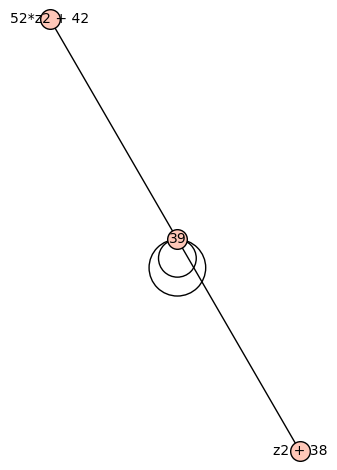
\includegraphics{../example_51_ordinary.png}
        \end{minipage}
        \begin{minipage}{0.5\textwidth}
            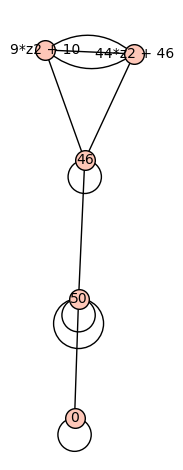
\includegraphics{../example_51_supersingular.png}
        \end{minipage}%
        \end{center}
        \caption{\label{fig:example_51} Ordinary 3-isogeny vulcano (left) and supersingular 3-isogeny graph (right) over $\F_{51^2}$, where $\mathrm{z2} = \alpha$ is a generator of $\F_{51^2}$.}
    \end{figure}
\end{example}
It is a fact that this example cannot completely show that the method works, and most roots are supersingular.
It would be much preferable with we could choose larger parameters, such that $\sqrt{p}$ and polynomial in $\log(p)$ look very different.
However, we very soon hit the limits of computers - just think that $\Phi_{3^4}$ already has 11162 monomials.

Also the standard approach using Groebner basis does not work, as we expect its complexity to be exponential in the number of variables, i.e. exponential in $\log_l(p)$.
Already for $l = 3$ and $e = 4$, it is very slow and takes time in the range of minutes.
The original paper~\cite{base_paper} thought it might be possible to use a ``square-and-multiply'' approach to compute the resultant
\begin{equation*}
    \mathrm{res}_Y(\Phi_n(X + \delta Y, X - \delta Y), \Phi_{l^e}(X + \delta Y, X - \delta Y))
\end{equation*} 
but this means we will not represent $\Phi_{l^e}$ by the polynomial system anymore, hence we would need to get enough information about the exponential-degree modular polynomial $\Phi_{l^e}$ another way.
This seems to be a very serious obstacle.

\section{An idea based on Sutherland's supersingularity test}
As an alternative to the above approach, we propose another set of polynomial equations, whose properties might make computations easier.
In particular, our system does not consist of long dependency cycles, in the sense that we have equations $f_i(x_i, x_{i + 1})$ and $f_n(x_n, x_0)$.
Instead, our equations are of the form $f_i(x_i, x_{i + 1})$ and $f_n(x_n)$, which seems to be easier to handle.

The basic idea is an observation by Sutherland \cite{sutherland_supersingularity_test}, namely that the lava flows of an ordinary vulcano can only have a bounded number of levels defined over $\F_{p^2}$.
Hence, we can consider the following algorithm, which is Sutherland's supersingularity test.
Beginning from the input j-invariant $j_0$, consider three random walks $j_0 = j_0^{(i)}, j_1^{(i)}, ..., j_n^{(i)}$ with $i \in \{ 1, 2, 3 \}$ in the $l$-isogeny graph of fixed length $n$ such that $j_1^{(1)}, j_1^{(2)}$ and $j_1^{(3)}$ are distinct.
Furthermore, assume the walks do not backtrack.
If $j_0$ is now ordinary, then at least one $j_1^{(i)}$ must be in a lava flow, and since the walks do not backtrack, one of them must descend in the corresponding lava flow tree.
For $n$ large enough, this shows that one $j_n^{(i)} \notin \F_{p^2}$.
On the other hand, the whole supersingular $l$-isogeny graph is defined over $\F_{p^2}$, so this will never happen.

It is easy to see that $n = \log_l(p)$ is sufficient, which is also Sutherland's original choice.
However, a slightly better bound can achieved, as observed by \cite{fp_supersingularity_tests}.
In our case, we are also interested in how many ordinary curves we will accept if we choose $n$ smaller than the optimal bound.
All this is considered in the next proposition.
\begin{theorem}
    \label{prop:counting_fp2_vulcano_levels}
    Let $p$ be an odd prime and $m \geq 2$ an odd integer coprime to $p$.
    Consider the number $n$ of endomorphism rings $\O$ of ordinary curves defined over $\F_{p^2}$ with $\pi \in \Z + m\O$, where $\pi$ is the $p^2$-Frobenius endomorphism
    \footnote{
        With the $p^2$-th power Frobenius endomorphism of an order $\O$, we mean a nontrivial element of norm $p^2$.
        There are at most two of them, and they are Galois conjugates. 
        Hence, for $\End(E) \cong \O$ we can choose an isomorphism such that $\pi$ is indeed mapped to the Frobenius. 
        Furthermore, by our study of the canonical isomorphism $\End(E) \cong \End(E')$ for isogeneous curves $E$ and $E'$, we know that the choice of the isomorphism $\O \cong \End(E)$ is compatible with all canonical isomorphisms.}
    of $\O$.
    Then
    \begin{equation*}
        \Bigl\lfloor \frac p {m^2} \Bigr\rfloor \leq n \leq \Bigl\lfloor \frac {4p(p + 1)} {m^3} \Bigr\rfloor
    \end{equation*}
    Furthermore, consider the number $N$ of ordinary j-invariants $j \in \F_{p^2}$ such that $\pi \in \Z + m\End(j)$.
    Under GRH, we then get
    \begin{equation*}
        c_1\left( \frac {p^2} {m^3 \log\log(p)^2} \right) \leq N \leq c_2\left( \frac {p^2\log(p)^2} {m^3} \right)
    \end{equation*}
    where $c_1, c_2 > 0$ are constants.
\end{theorem}
\begin{proof}
    First, we show the lower bounds.
    Note that there are $\lfloor p/m^2 \rfloor$ different integers $a$ with $0 < am^2 < p$ (clearly $m^2 \notdivides p$).
    For each of them, consider $D = 4am^2(am^2 - p)$.
    Clearly $D$ is a fundamental discriminant, as $D \equiv 0 \mod 4$.
    We have
    \begin{equation*}
        (p - 2am^2)^2 - D \cdot 1^2 = p^2 - 4pam^2 + 4a^2m^4 - 4a^2m^4 + 4pam^2 = p^2
    \end{equation*}
    Thus the imaginary quadratic order $\O$ with discriminant $D$ contains a nontrivial element of norm $p^2$, which must be the Frobenius $\pi$.
    In particular, the imaginary quadratic order $\O_0$ with discriminant $d := D/m^2$ satisfies $\O = \Z + m\O_0$ as $[\O_0 : \O]^2 = d(\O)/d(\O_0) = m^2$
    Therefore we see that $\pi \in \Z + m\O_0$.
    Note that each $a$ gives rise to a distinct $\O_0$, and the first lower bound follows.

    To get a lower bound for the number of curves, note that for each $\O_0$, by the class group action, there are exactly $\#\Cl(\O_0)$ such curves.
    Under GRH, Thm~\ref{prop:class_number_bounds} gives
    \begin{equation*}
        h(d) \geq \frac {\sqrt{|d|}} {(\log\log|d|)^2} \Theta(1)
    \end{equation*}
    Hence, the total number of curves is lower bounded by
    \begin{align*}
        &\Theta(1) \sum_{1 \leq a \leq \lfloor p/m^2 \rfloor} h(4a(am^2 - p)) \geq \Theta(1) \sum_{1 \leq a \leq \lfloor p/m^2 \rceil} \frac {\sqrt{4a|am^2 - p|}} {(\log\log|4a(am^2 - p)|)^2} \\
        =& \Theta(1) m \sum_{1 \leq a \leq \lfloor p/m^2 \rfloor} \frac {\sqrt{a} \sqrt{p/m^2 - a}} {(\log(\log(4) + \log(am^2) + \log(p - am^2)))^2} \\
        \geq& \Theta(1) \frac {m} {(\log(\log(4) + 2\log(p/2)))^2} \sum_{1 \leq a \leq \lfloor p/m^2 \rfloor} \sqrt{a} \sqrt{p/m^2 - a} \\
        =& \Theta(1) \frac {m} {\log\log(p)^2} \int_0^{p/m^2} \sqrt{a} \sqrt{p/m^2 - a} \ da \\
        =& \Theta(1) \frac {p^2} {m^3 \log\log(p)^2} \int_0^1 \sqrt{x(1 - x)} dx = \Theta\left( \frac {p^2} {m^3 \log\log(p)^2} \right)
    \end{align*}
    We assume that $p \geq m^2$ when estimating the sum by the integral.

    Now to the upper bounds.
    Consider an endomorphism ring $\O_0$ such that $\O := \Z + m\O_0$ contains the $p^2$-Frobenius $\pi$.
    Then
    \begin{equation*}
        \Z[\pi] \subseteq \O \subseteq \O_0
    \end{equation*}
    and so $D := d(\Z[\pi]) = a^2m^2d(\O_0)$.
    Furthermore, if $t$ is the trace of $\pi$, we find $D = t^2 - 4p^2 = (t - 2p)(t + 2p)$.
    Hence
    \begin{equation*}
        a^2m^2d(\O_0) = (t - 2p)(t + 2p)
    \end{equation*}
    Unless $m = 2$ or $m = 4$, $m$ cannot divide both $t - 2p$ and $t + 2p$.

    If $m^2 \divides t + 2p$, then $t \in \{ m^2 - 2p, 2m^2 - 2p, ..., km^2 - 2p \}$ where $k = \lfloor 2p/m^2 \rfloor$.

    If $m^2 \divides t - 2p$, then $t \in \{ 2p - (k + 1)m^2, 2p - (k + 2)m^2, ..., 2p - (2k + 1)m^2 \}$.
    \\
    In particular, there are at most $2k + 1$ different choices for $t$.
    For a given $t$, there are now at most
    \begin{equation*}
        \sqrt{\frac {|t^2 - 4p^2|} {m^2}} \leq \sqrt{\frac {4p^2} {m^2}} = \frac {2p} m
    \end{equation*}
    choices for $a$, which then uniquely determines $d(\O_0)$.
    The total number of possibilities for $d(\O_0)$ is thus
    \begin{equation*}
        (2k + 1) \frac {2p} {m} \leq \frac {4p(p + 1)} {m^3}
    \end{equation*}
    To bound the number of curves, we again use the class group action and the following bound on the class number of a quadratic imaginary number field.
    Namely, if the discriminant is $d$, have
    \begin{equation*}
        h(d) \leq \sqrt{|d|}\log(|d|) O(1)
    \end{equation*}
    This now gives us the following upper bound on the number of curves
    \begin{align*}
        &\sum_{1 \leq i \leq k} \quad \sum_{a^2 \divides ((im^2 - 2p)^2 - 4p^2)/m^2} h\Biggl( \frac {(im^2 - 2p)^2 - 4p^2} {a^2m^2} \Biggr) \\
        &+ \sum_{k + 1 \leq i \leq 2k + 1} \quad \sum_{a^2 \divides ((2p - im^2)^2 - 4p^2)/m^2} h\Biggl( \frac {(2p - im^2)^2 - 4p^2} {a^2m^2} \Biggr) \\
        \leq& O(\log(4p^2/m^2)) \Biggl( \sum_{1 \leq i \leq k} \sqrt{\frac {4p^2 - (im^2 - 2p)^2} {m^2}} \sum_{a^2 \divides ((im^2 - 2p)^2 - 4p^2)/m^2} \frac 1 a \\
        &+ \sum_{k + 1 \leq i \leq 2k + 1} \sqrt{\frac {4p^2 - (2p - im^2)^2} {m^2}} \sum_{a^2 \divides ((2p - im^2)^2 - 4p^2)/m^2} \frac 1 a \Biggr)
    \end{align*}
    Note that
    \begin{align*}
        \sum_{a^2 \divides x} \frac 1 a \leq \sum_{a \leq \sqrt{x}} \frac 1 a = O(\log(x))
    \end{align*}
    Thus we can upper bound the previous sum by
    \begin{align*}
        &O(\log(4p^2/m^2)) \Biggl( \sum_{1 \leq i \leq k} \sqrt{ \frac {4p^2 - (im^2 - 2p)^2} {m^2}} \quad \log\left( \frac {4p^2 - (im^2 - 2p)^2} {m^2} \right) \\
        &+ \sum_{k + 1 \leq i \leq 2k + 1} \sqrt{ \frac {4p^2 - (2p - im^2)^2} {m^2}} \quad \log\left( \frac {4p^2 - (2p - im^2)^2} {m^2} \right) \Biggr) \\
        \leq& \frac {O(\log(p/m)^2)} {m} \Biggl( \sum_{1 \leq i \leq k} \sqrt{4p^2 - (im^2 - 2p)^2} + \sum_{k + 1 \leq i \leq 2k + 1} \sqrt{4p^2 - (2p - im^2)^2} \Biggr) \\
        =& \frac {O(\log(p/m)^2)} {m} \Biggl( \int_0^k \sqrt{4p^2 - (xm^2 - 2p)^2} dx + \int_{k + 1}^{2k + 2} \sqrt{4p^2 - (xm^2 - 2p)^2} dx \Biggr) \\
        \leq& \frac {O(\log(p/m)^2)} {m} \Biggl( \int_0^k \sqrt{4p^2 - (xm^2 - 2p)^2} dx + \int_{k}^{2k} \sqrt{4p^2 - (xm^2 - 2p)^2} dx + O(p) \Biggr) \\
        =& \frac {O(\log(p/m)^2)} {m} \Biggl( \frac 1 {m^2} \int_0^{2p} \sqrt{4p^2 - (x - 2p)^2} dx + \frac 1 {m^2} \int_{2p}^{4p } \sqrt{4p^2 - (2p - x)^2} dx + O(p)\Biggr) \\
        =& \frac {O(\log(p/m)^2)} {m} \Biggl( \frac 1 {m^2} \int_{-2p}^0 \sqrt{4p^2 - x^2} dx + O(p) \Biggr) \\
        =& \frac {O(\log(p/m)^2)} {m} \Biggl( \frac {4p^2} {m^2} \int_{-1}^0 \sqrt{1 - x^2} \Biggr) = O\left( \frac {p^2\log(p/m)^2} {m^3} \right)
    \end{align*}
    This shows the claim.
\end{proof}
In particular, it follows that we can choose $m = l^r$ with $r = \lceil \frac 1 2 \log_l(p) \rceil$ and can be sure never to accept an ordinary curve as supersingular.
Furthermore, if we are ok with accepting $O(p)$ ordinary curves as supersingular, we can choose $r = \lceil \frac 1 3 \log_l(p) \rceil$.

\subsection{Generating curves}
According to the above discussion, the obvious polynomial system we want to find a root of is
\begin{equation*}
    \langle \Phi_m(x, y_1), \Phi_m(x, y_2), \Phi_m(x, y_3), \ y_1^{p^2 - 1} - 1, \ y_2^{p^2 - 1} - 1, \ y_3^{p^2 - 1} - 1 \rangle
\end{equation*}
Since $m$ will be exponentially large, and we thus have no good description of $\Phi_m$, we can instead consider the paths explicitly again.
More concretely, consider the polynomial system
\begin{align*}
    \langle &\Phi_l(x, u_0), \Phi_l(x, v_0), \Phi_l(x, w_0), \\
    &\Phi_l(u_0, u_1), \Phi_l(v_0, v_1), \Phi_l(w_0, w_1), \\
    &... \\
    &\Phi_l(u_{n - 1}, u_n), \Phi_l(v_{n - 1}, v_n), \Phi_l(w_{n - 1}, w_n), \\
    &u_n^{p^2 - 1} - 1, v_n^{p^2 - 1} - 1, w_n^{p^2 - 1} - 1 \rangle
\end{align*}
We can explicitly write down that system.

However, a solution to this system might ``collapse'' nodes, e.g. have $u_i = u_{i + 2}$.
Then the corresponding $l$-isogeny path backtracks, and it is not guaranteed that one path reaches the $n$-th lava flow level.
Hence, we can still get many ordinary curves.

Then condition $u_i \neq u_{i + 2}$ is not algebraically closed, so we cannot write it as a polynomial directly.
But we can use the structure of the vulcanos (in particular, they have at most one cycle), and the fact that $\Phi_m$ characterizes the existence of a \emph{cyclic} isogeny.
Hence, consider the polynomial system
\begin{align*}
    \langle &\Phi_l(x, u_0), \Phi_l(x, v_0), \Phi_l(x, w_0), \\
    &\Phi_l(u_0, u_1), \Phi_l(v_0, v_1), \Phi_l(w_0, w_1), \\
    &... \\
    &\Phi_l(u_{n - 1}, u_n), \Phi_l(v_{n - 1}, v_n), \Phi_l(w_{n - 1}, w_n), \\
    &u_n^{p^2 - 1} - 1, v_n^{p^2 - 1} - 1, w_n^{p^2 - 1} - 1, \\
    &\Phi_{l^2}(u_0, v_0), \Phi_{l^2}(u_0, w_0), \Phi_{l^2}(v_0, w_0), \\
    &\Phi_{l^2}(u_0, u_2), \Phi_{l^2}(v_0, v_2), \Phi_{l^2}(w_0, w_2), \\
    &... \rangle
\end{align*}
The additional constraints $\Phi_{l^2}(u_i, u_{i + 2})$ ensure that $u_i \neq u_{i + 2}$, unless the curve of j-invariant $u_i$ has a cyclic endomorphism of size $l^2$.
However, this means that its endomorphism ring has polynomially large discriminant, and by the class group action, there are only polynomially many such curves.
Hence, a root of above system is supersingular with probability $1 - 1/\mathrm{poly}(\log(p))$. 

Still, it seems pretty impossible to efficiently compute a random root of above system.
We now present a way that looks like there is some hope to do the computations, even though there are still some serious obstacles.
\begin{prop}
    Let $\O$ be an order in a quadratic imaginary number field with $p^2$-power Frobenius $\pi$.
    Let $l_1, ..., l_r$ be distinct primes.
    Then
    \begin{equation*}
        \pi \in \Z + l_1 ... l_r \O \quad \Leftrightarrow \quad \forall i: \pi \in \Z + l_i \O
    \end{equation*}
\end{prop}
\begin{proof}
    The direction $\Rightarrow$ is clear, as $\Z + l_1 ... l_r \O \subseteq \Z + l_i\O$.
    For the other direction, choose an integral generator $\alpha$ of $\O$, i.e. $\O = \Z + \alpha\Z$.
    Then $\Z + l_i\O = \Z + l_i\alpha\Z$.
    Furthermore, there is a unique representation $\pi = a + b\alpha$.
    Now the assumption
    \begin{equation*}
        \pi \in \Z + l_i\O = \Z + l_i\alpha\Z
    \end{equation*}
    implies $l_i \divides b$, and so $l_1 ... l_r \divides b$.
    Thus
    \begin{equation*}
        \pi \in \Z + l_1 ... l_r \O = \Z + l_1 ... l_r \alpha \Z \qedhere
    \end{equation*}
\end{proof}
Hence, we can instead consider the sum of systems
\begin{align*}
    \sum_i \quad \langle &\Phi_{l_i}(x, u_i), \Phi_{l_i}(x, v_i), \Phi_{l_i}(x, w_i), \\
    &\Phi_{2l_i}(u_i, v_i), \Phi_{2l_i}(u_i, w_i), \Phi_{2l_i}(v_i, w_i), \\
    &u_i^{p^2 - 1} - 1, v_i^{p^2 - 1} - 1, w_i^{p^2 - 1} - 1 \rangle 
\end{align*}
for distinct primes $l_i$ with $\prod_i l_i \geq \sqrt{p}$.
Finally, we can still make it somewhat more explicit.
\begin{lemma}
    Assume that $k$ is an algebraically closed field.
    Let $I \leq k[x, Y, B]$ be an ideal, where $Y$ and $B$ are vectors of unknowns.
    Then elimination and evaluation commute, i.e.
    \begin{equation*}
        \mathrm{ev}_{x, b}(I \cap k[x, B]) = \mathrm{ev}_{x, Y, b}(I) \cap k[x]
    \end{equation*}
    where $b \in k[x]^n$ is a vector and $\mathrm{ev}_{x, b}$ resp. $\mathrm{ev}_{x, Y, b}$ are evaluation homomorphisms.
\end{lemma}
\begin{proof}
    Taking the point of view of varieties over the algebraically closed field $k$, we see that elimination corresponds to projection (the main theorem of elimination theory), and evaluation corresponds to the intersection with a linear subspace.
    Clearly, both of them commute in the above sense.
\end{proof}
\begin{lemma}
    \label{prop:symbolic_elimination}
    We have
    \begin{equation*}
        y^{p^2 - 1} - 1 \equiv \left(\begin{matrix*}
            y^l \\
            \vdots \\
            1
        \end{matrix*}\right)^T b - 1 \mod \Phi_l(x, y)
    \end{equation*}
    where
    \begin{equation*}
        b = A^{p^2 - l - 1} e_1 \quad \text{for the first unit vector $e_1 = \left(\begin{matrix*}
            1 \\
            0 \\
            \vdots \\
            0
        \end{matrix*}\right)$}
    \end{equation*}
    for the explicitly computable $(l + 1) \times (l + 1)$ matrix $A \in k[x]^{(l + 1) \times (l + 1)}$ given by
    \begin{equation*}
        A = \left( \begin{matrix*}
            -a_l & 1 & 0 & \dots & 0 \\
            -a_{l - 1} & 0 & 1 & \dots & 0 \\
            \vdots & \vdots & \vdots & \ddots & \vdots \\
            -a_1 & 0 & 0 & \dots & 1 \\
            -a_0 & 0 & 0 & \dots & 0
        \end{matrix*} \right) \in k[x]^{(l + 1) \times (l + 1)}
    \end{equation*}
    where
    \begin{equation*}
        \Phi_l(x, y) = \sum_{i = 0}^{l + 1} a_i(x) y^i \in k[x][y]
    \end{equation*}
    as univariate polynomial over $k[x]$.
\end{lemma}
\begin{proof}
    We just perform univariate polynomial division of $y^{p^2 - 1} - 1$ by $\Phi_l(x, y)$ in $k[x][y]$.

    Define a sequence of polynomials in $k[x, y]$ by
    \begin{equation}
        f_0 := y^{p^2 - 1} \quad \text{and} \quad f_{i + 1} = f_i - \mathrm{lc}(f_i) \Phi_l(x, y) y^{p^2 - l - 2 - i}
    \end{equation}
    Here, $\mathrm{lc}(f_i)$ and $\deg$ refer to the appropriate values when considering $f_i$ as a univariate polynomial over $k[x]$, in particular $\mathrm{lc}(f_i) \in k[x]$.
    This clearly implies that $f_i \equiv f_j \mod \Phi_l(x, y)$.
    We show that
    \begin{equation*}
        f_i = \left( \begin{matrix*}
            y^{p^2 - 1 - i} \\ \vdots \\ y^{p^2 - l - 1 - i}
        \end{matrix*} \right)^T A^i e_1
    \end{equation*}

    To see that this is true, note that $f_i$ has contains only the monomials $y^{p^2 - 1 - i}, ..., y^{p^2 - l - 1 - i}$ (technically, by induction hypothesis).
    Hence, we can write
    \begin{equation*}
        f_i = y^{p^2 - l - 1 - i} \sum_{j = 0}^l c_j y^j
    \end{equation*}
    Since $a_{l + 1} = 1$, it follows that
    \begin{align*}
        f_{i + 1} =& y^{p^2 - l - 1 - i} \Bigl( \sum_{j = 0}^l c_j - c_l a_{j + 1} \Bigr) - y^{p^2 - l - 2 - i} c_l a_0 \\
        =& y^{p^2 - l - 1 - (i + 1)} \sum_{j = 0}^l (c_{j - 1} - c_l a_j)
    \end{align*}
    where we define $c_{-1} = 0$.
    Now we have
    \begin{equation*}
        \left( \begin{matrix*}
            c_{l - 1} - c_l a_l \\
            \vdots \\
            c_0 - c_l a_1 \\
           - c_l a_0
        \end{matrix*} \right) = A \left( \begin{matrix*}
            c_l \\
            \vdots \\
            c_1 \\
            c_0
        \end{matrix*} \right)
    \end{equation*}
    and the claim follows.
\end{proof}
The idea is now to introduce $l + 1$ indeterminates $B$, and compute the elimination ideal
\begin{align*}
    \langle &\Phi_{l_i}(x, u_i), \Phi_{l_i}(x, v_i), \Phi_{l_i}(x, w_i), \\
    &\Phi_{2l_i}(u_i, v_i), \Phi_{2l_i}(u_i, w_i), \Phi_{2l_i}(v_i, w_i), \\
    &\left(\begin{matrix*}
        u_i^l \\
        \vdots \\
        1
    \end{matrix*}\right)^T B - 1, \left(\begin{matrix*}
        v_i^l \\
        \vdots \\
        1
    \end{matrix*}\right)^T B - 1, \left(\begin{matrix*}
        w_i^l \\
        \vdots \\
        1
    \end{matrix*}\right)^T B - 1 \rangle \cap k[x, B]
\end{align*}
Now we can find polynomials $f_{i1}, ..., f_{in_i} \in k[x, B]$ that generate this ideal.
Hence, we only have to find a random joint root of the univariate polynomials
\begin{equation*}
    f_{ij}(x, b_i) \quad \text{where} \quad b_i = A_i^{p^2 - l - 1} e_1
\end{equation*}
for the matrices $A_i$ given by Lemma~\ref{prop:symbolic_elimination}.
While we cannot explicitly write down those polynomials, we can evaluate them, evaluate their derivates and perform a series of other computations.
Hence, there might be some way to find a random root of those (note that they have all $\Theta(p/12)$ supersingular j-invariants and some $o(p)$ ordinary j-invariants as roots).

